\chapter{Wykład 11. Zarządzanie jakością w projekcie informatycznym}

\section{Lista kontrolna}
% strona 38

\textbf{Obszar projektu:} ocena wiarygodności estymacji harmonogramu i kosztu projektu

\begin{figure}[h]
\begin{center}
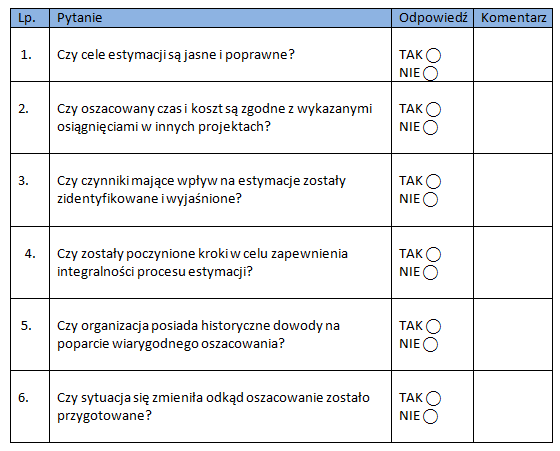
\includegraphics[scale=1]{checklist.png}
\caption[Lista kontrolna]{Lista kontrolna}
\label{rysunekProces}
\end{center}
\end{figure}

% ===========================================================================

\section{Plan poprawy procesów}
% strona 39

\textbf{Obszar projektu:} komunikacja

\textbf{Problem:} zespół nie może się dogadać, wymagania dotyczące projektu są błędnie interpretowane przez różne osoby, błędy jednej osoby pociągają za sobą błędy kolejnych, błędny przepływ informacji.

\textbf{Cel:} zgrany zespół, wymieniający się informacjami i problemami posiadający jasno określony cel działania znany wszystkim członkom zespołu

\begin{figure}[h]
\begin{center}
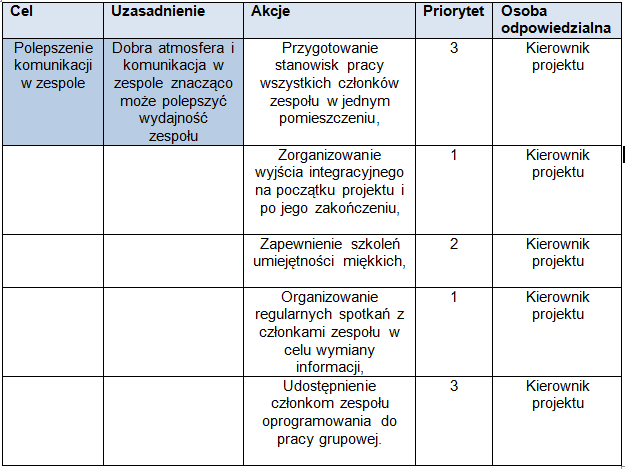
\includegraphics[scale=1]{planpoprawy.png}
\caption[Plan poprawy procesu]{Plan poprawy procesu}
\label{rysunekProces}
\end{center}
\end{figure}
 


% ===========================================================================

\section{Plan zarządzania jakością pod kątem przydziału zasobów}
% strona 56

\begin{enumerate}
\item	Przygotowanie listy wszystkich zasobów na podstawie RBS.
\item	Bieżąca ocena zasobów ludzkich pod kątem kwalifikacji i stanowiska.  Sprawdzenie czy pracownicy wypełniają swoje obowiązki zawarte w opisie stanowiska oraz czy ich kwalifikacje pozwalają na wykonywanie danych czynności.
\item	Kontrola czy zasoby nie są przeciążone – czy nie jest im przypisane zbyt dużo pracy do wykonania, czy nie są zbyt eksploatowane.
\end{enumerate}

% ===========================================================================

\section{Audyt jakości}
% strona 62

Ten wirtualny warsztat jest beznadziejny.

% ===========================================================================

\section{Wyniki procesu kontroli jakości}
% strona 68
Dzięki audytowi możliwa jest kontrola procesów mających miejsce w przedsiębiorstwie. Audyty pozwalają na wykrycie niedoskonałości i błędów w działaniu. Każdy naprawiony defekt i dostarczony produkt również musi przejść przez kontrolę jakości. 

Dokument wyniku procesu kontroli mógłby wyglądać w następujący sposób:

\begin{figure}[h]
\begin{center}
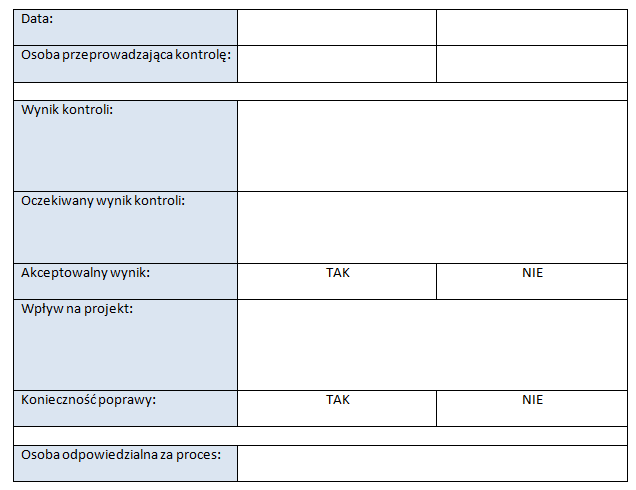
\includegraphics[scale=1]{wyniki.png}
\caption[Szablon dokumentu]{Szablon dokumentu}
\label{rysunekProces}
\end{center}
\end{figure}

% ===========================================================================

\section{Diagram przyczynowo-skutkowy w zarządzaniu jakością}
% strona 80

Diagram przyczynowo-skutkowy jest jednym z narzędzi doskonalenia jakości. Pozwala na zidentyfikowanie przyczyny problemu i ułatwia znaleznienie przyczyny źródłowej problemu (root cause). Etapy tworzenia:
\begin{enumerate}
\item	Identyfikacja problemu (szary prostokąt).
\item	Określenie głównych grup przyczyny (niebieskie prostokąty)
\item	Uszczegółowienie przyczyn 
\item	Analiza wyników.
\end{enumerate}

\begin{figure}[h]
\begin{center}
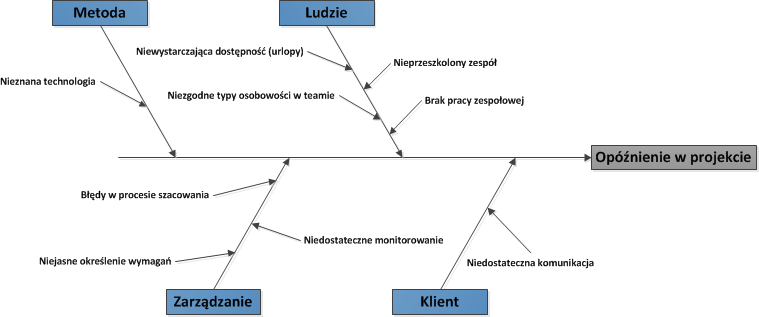
\includegraphics[scale=0.8]{ryba.png}
\caption[Diagram przyczynowo-skutkowy]{Diagram przyczynowo-skutkowy}
\label{rysunekProces}
\end{center}
\end{figure}



% ===========================================================================

\section{Diagram Pareto}
% strona 83

\begin{figure}[h]
\begin{center}
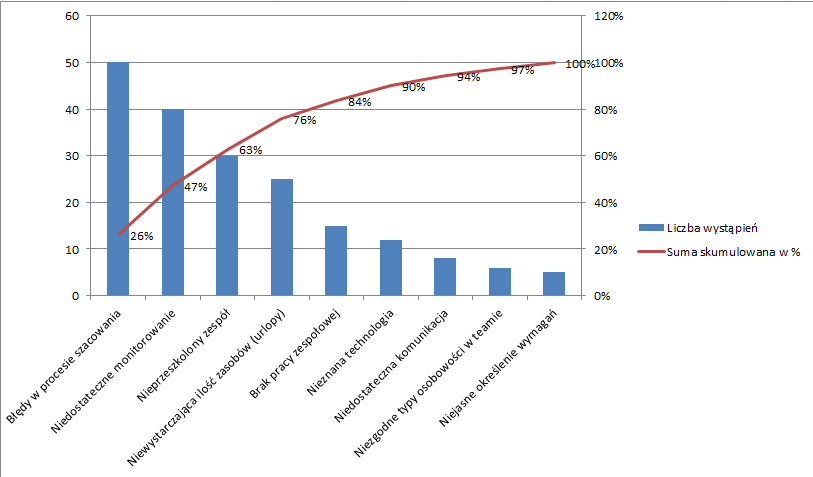
\includegraphics[scale=0.8]{pareto.png}
\caption[Diagram Pareto]{Diagram Pareto}
\label{rysunekProces}
\end{center}
\end{figure}


Czy zasada 20-80 się sprawdza?

W wykonanym przykładzie zasada 20-80 nie sprawdziła się.  Około 80\% problemów było generowanych przez ok 44\% przyczyn.



